\documentclass[tikz,margin=1mm]{standalone}

\def\fact{.4}
\usetikzlibrary{calc}
\begin{document}

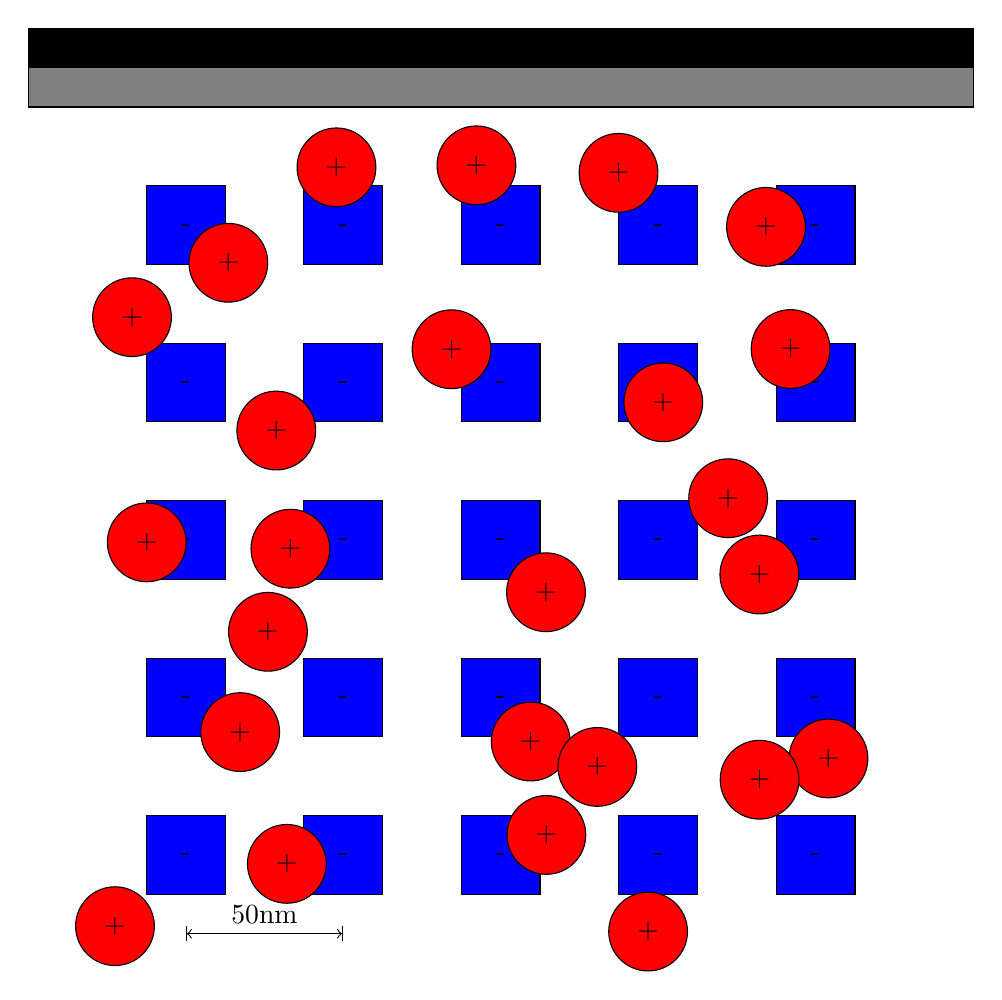
\begin{tikzpicture} % problem with scaling is text doesn't scale with it
%% dopant "lattices" (simplification)
\foreach\x in {1,2,3,4,5}
  \foreach\y in {-1,-2,-3,-4,-5}
    {
    \node[draw, minimum size=1cm, fill=blue] at (2*\x,2*\y) {-};
    }
\foreach\x in {1,2,3,4,5}
  \foreach\y in {-1,-2,-3,-4,-5} 
    {
    \node[draw, circle, minimum size=1cm, fill=red] at ($(2*\x, 2*\y) + (rand,rand)$) {+};
    }

\draw[fill=gray] (0, -.5) rectangle (12, 0);
% 1 cm = 50 nm (see length scale), tox ~=25 nm
\draw[fill=black] (0, 0) rectangle (12, .5);

% scale bar
\draw[|<->|] (2, -11) -- (4, -11) node[pos=0.5, above] {50nm};

\end{tikzpicture}
%
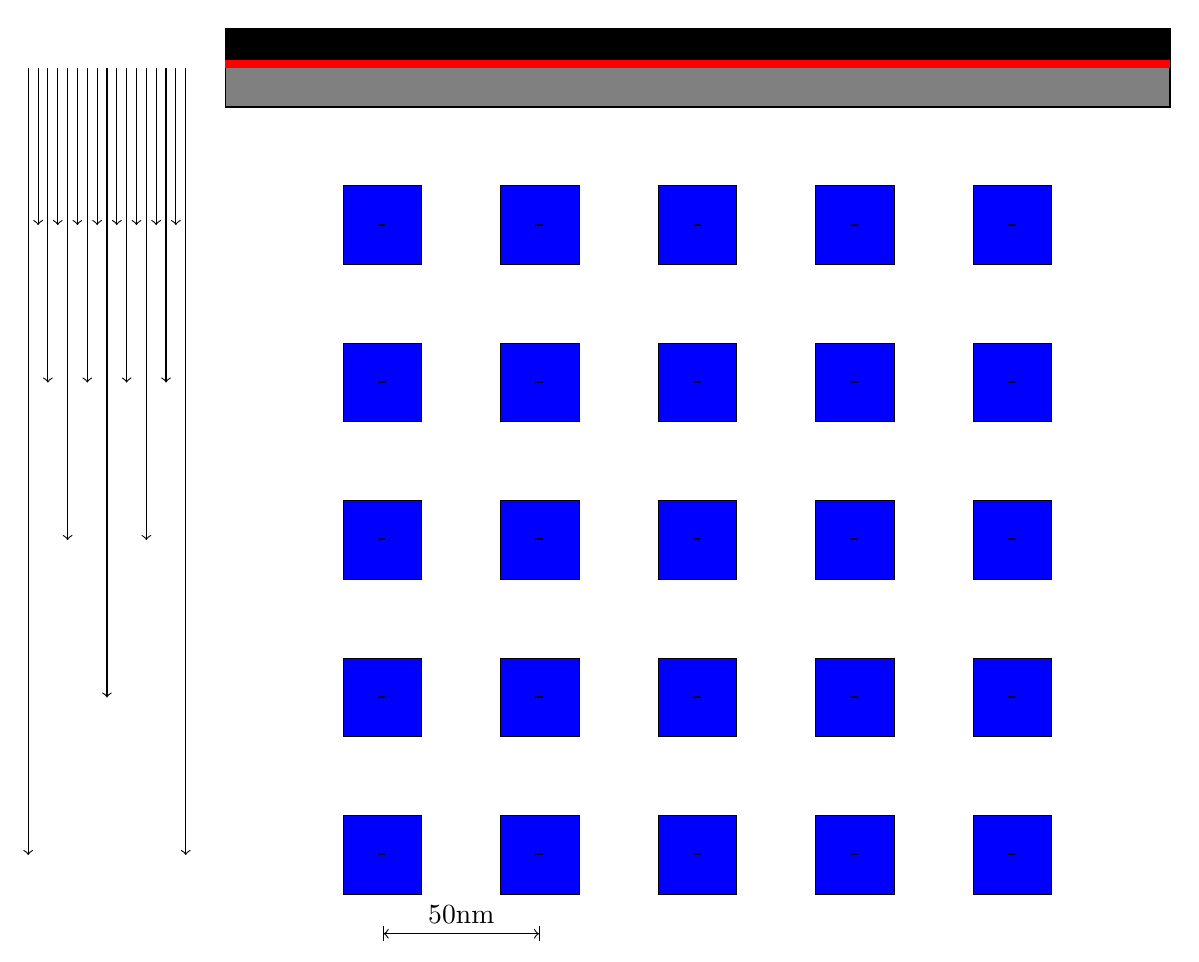
\begin{tikzpicture} % problem with scaling is text doesn't scale with it
%% dopant "lattices" (simplification)
\foreach\x in {1,2,3,4,5}
  \foreach\y in {-1,-2,-3,-4,-5}
    {
    \node[draw, minimum size=1cm, fill=blue] at (2*\x,2*\y) {-};
    }

\draw[fill=gray] (0, -.5) rectangle (12, 0);
% 1 cm = 50 nm (see length scale), tox ~=25 nm
\draw[fill=black] (0, 0) rectangle (12, .5);
\fill[fill=red] (0,0) rectangle (12, .1);

% scale bar
\draw[|<->|] (2, -11) -- (4, -11) node[pos=0.5, above] {50nm};

\begin{scope}[xshift=2.5cm]
\draw[->] (-5, 0) -- (-5, -10);
\draw[->] (-3, 0) -- (-3, -10);
% first bisection
\draw[->] (-4, 0) -- (-4, -8);
% second bisection
\draw[->] (-4.5, 0) -- (-4.5, -6);
\draw[->] (-3.5, 0) -- (-3.5, -6);
% third bisection
\draw[->] (-4.25, 0) -- (-4.25, -4);
\draw[->] (-4.75, 0) -- (-4.75, -4);
\draw[->] (-3.75, 0) -- (-3.75, -4);
\draw[->] (-3.25, 0) -- (-3.25, -4);
% fourth bisection
\draw[->] (-3.125, 0) -- (-3.125, -2);
\draw[->] (-3.375, 0) -- (-3.375, -2);
\draw[->] (-3.625, 0) -- (-3.625, -2);
\draw[->] (-3.875, 0) -- (-3.875, -2);
\draw[->] (-4.125, 0) -- (-4.125, -2);
\draw[->] (-4.375, 0) -- (-4.375, -2);
\draw[->] (-4.625, 0) -- (-4.625, -2);
\draw[->] (-4.875, 0) -- (-4.875, -2);
%
\end{scope}

\end{tikzpicture}

\end{document}
